\section{Data Reduction Overview}
\label{sec:overview}

The \instrument{} pipeline, like most other recent ESO instrument pipelines, can be executed in three different ways: with \emph{Gasgano}, \emph{esorex} and \emph{Reflex}.
Although these are somewhat different environments, it is always the
same pipeline, as far as pipeline recipes are concerned.
Gasgano
is a FITS-file browser and running the pipeline this way is a ``manual'' task, typically good only for quick look checks.

Reflex executes the recipes via graphic workflow interface which has advantages like sorting data and finding the necessary calibrations
automatically, and keeping track of previous executions. 
The reflex workflows are described in the Reflex Tutorial while this manual uses esorex in its examples on how to run the data reduction cascade.

The details on recipe algorithms and parameters are contained in this document, and the Reflex workflows reduce the calibrations as described in Ch.~\ref*{sec:simcalexpl}, before executing one of the science recipes (Ch.~\ref*{sec:sci-reduc}).


\subsection{Data Formats}
\label{sec:data-fmt-quick}

\subsubsection{Detectors and Extensions}
\label{sec:extns}
\begin{figure}[!tb]
  \begin{center}
    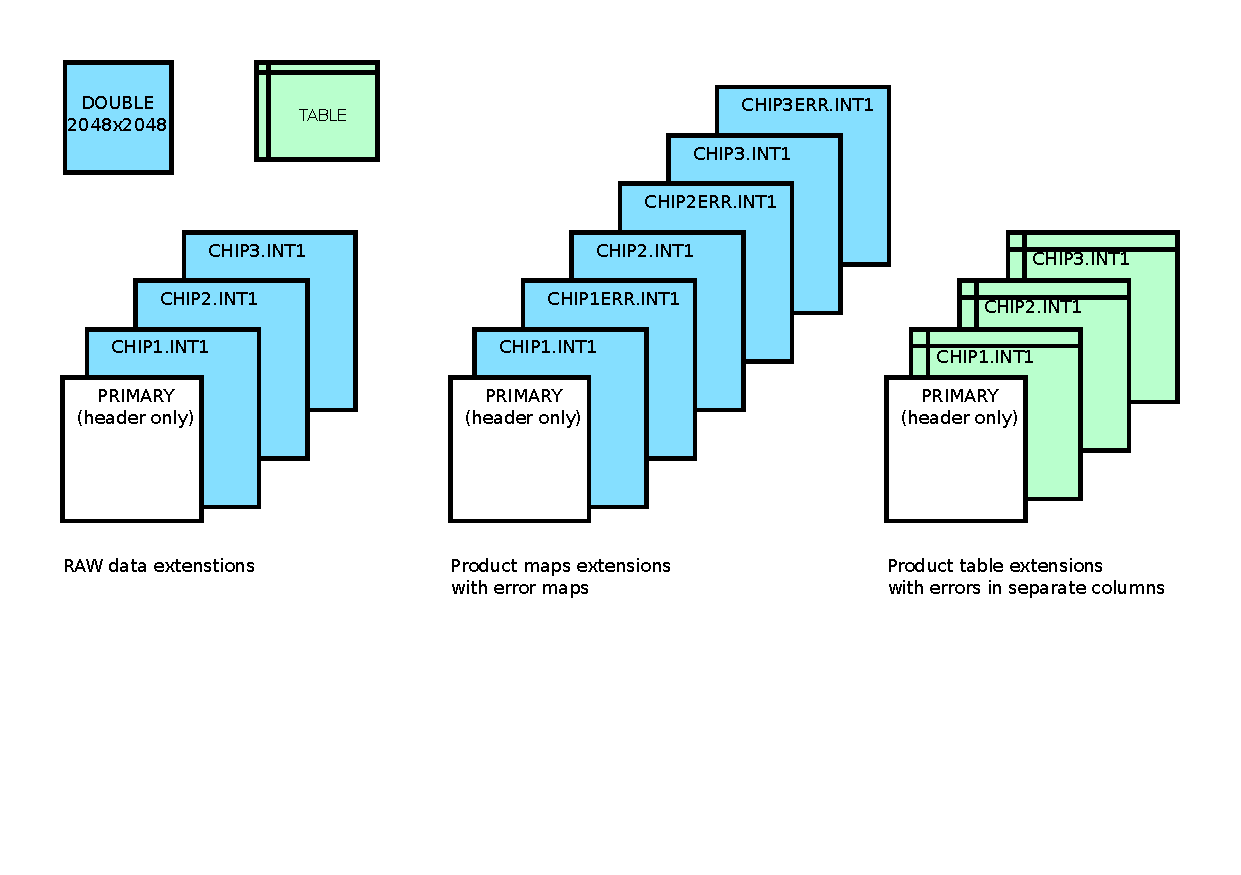
\includegraphics[width=0.99\linewidth]{fits_ext.pdf}
  \end{center}
  \caption{
    \label{fig:fits_ext}
    FITS extensions in raw frames and data products.
    }
\end{figure}

Raw data comes as FITS files that contain only headers in the primary extension,
and one image extension with the readout result from each detector. The latter
are named like \verb!CHIPn.INT1! where \texttt{n} is the detector number (1…3),
in order from left to right with increasing wavelength in each spectral order.

Data reduction products are either FITS tables or images, depending on whether
the product is an image/map or not. The separation into extensions of data from
the three detectors is kept, and most recipes treat them independently. For
derived maps or images that have errors, three more extension are present, named
like \texttt{CHIPnERR.INT1}.

Fig.~\ref{fig:fits_ext} illustrates this. The extensions are usually ordered,
however we recommend to not rely on the index when opening files with custom
scripts or tools. Instead, the FITS extension \emph{name} should be used.


\subsubsection{Data Product Headers}

The DRS recipes use the FITS headers of the \emph{first raw file} in the SOF as
basis for the data products' headers.

Recipes also add some new headers:

\begin{itemize}
    \item The header keys specific to the data product are named \verb!PRO.*! and includes classification (\verb!PRO.TYPE!, \verb!PRO.CATG!), the list of input files (\verb!PRO.RECi,RAWj! and \verb!PRO.RECi.CALIBj!), and recipe parameters and their values (\verb!PRO.RECi.PARAMj!); with \verb!i,j! being integers increasing from $1$.
    \item Named \verb!QC.*! are the results of quality control parameters, which are used for instrument monitoring. Note that these often reside in the extension headers, since they are derived for each detector.
\end{itemize}

\subsubsection{The TraceWave-Table}
\label{sec:tracewave}

\begin{figure}[!tb]
    \begin{center}
      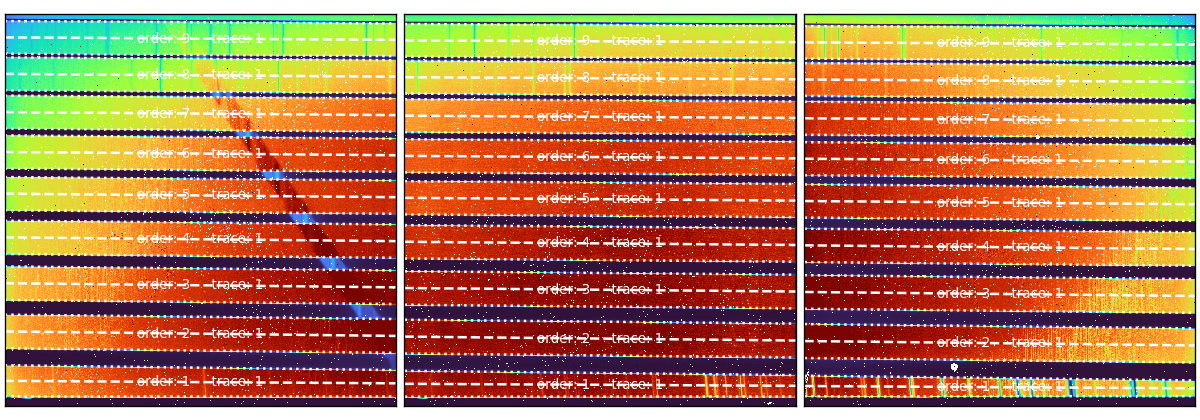
\includegraphics[width=0.99\linewidth]{J_2_3_03_cr2res_util_trace_out.png}
    \end{center}
    \caption{
      \label{fig:flat_trace}
      An example of a raw flat-field frame in J1228. Overplotted in white is 
      the result of the order tracing, the polynomial fit to the mid-line
      (dashed) and edges (dotted) for each detector-order.
      }
  \end{figure}

The most important FITS table within the \instrument\ DRS is the
\emph{TraceWave}, abbreviated TW henceforth. It contains information about how
spectral orders are located in the detectors' pixel grid, how the projection of
the slit changes, and the wavelength solution.

Each row in the table corresponds to a single \emph{trace}. Each trace belongs
to a single spectral order; an order can have one or more traces, numbered
starting with 1 within each order. The \emph{order number} and \emph{trace
number} are two of the columns in the TW table, and together they uniquely
identify a trace, i.e.~a table row.

Each trace stores three polynomials: one for the mid-line, upper and lower edge,
respectively. Polynomials are stored as coefficients, lowest power first, and
evaluated for pixel columns starting with index 1. Fig.~\ref{fig:flat_trace}
shows these polynomials plotted onto a flat-field frame. Associated with each
trace is also its \emph{slit-fraction}, that is a number $[0.0\ldots 1.0]$ which
indicates the height along the slit, ranging from $0.0$ at the bottom to $1.0$
at the top. Three values are provided, one each for lower edge, mid-line and
upper edge of the trace, so that a trace for the full slit has
\verb!SlitFraction=[0.0,0.5,1.0]!. Partial slit-fractions are used for nodding
and polarimetry; see also Ch.~\ref{sec:slitfracbinary}.

Analogous to traces, the wavelength solution is stored as polynomial coefficients
that represent the translation from pixel to wavelength space. Because the slit
is not vertical with respect to the pixel columns, the wavelength scale
naturally shifts within each spectral order. This is taken into account when the
spectra are extracted, so that the TW only needs to store the wavelength
solution at the mid-line of the trace.

How the orientation and shape of the slit changes along each trace is saved as
three "meta-polynomials" that are described in detail in Ch.~\ref{sec:tilt}.
Since this is handled automatically by the extraction methods, users normally
should not need to get familiar with this aspect.

Several recipes take a TW as input and produce a new one, with some information
updated. Notably the wavecal recipe needs a TW as input to know how to extract
the spectra of the calibration lamps, and to get a first-guess of the
wavelength solution; it will then output a TW with the new wavelengths and
the other information propagated from the input.

Naturally, each TW is specific to a single standard setting of the spectrograph.
The order tracing and slit tilt are expected to be stable enough to be re-used
between nights, especially for observations taken with metrology turned on. The
limiting factor is the repeatability of the echellogram (cf.~User Manual), but
the DRS should not fail to reduce even with significantly mismatched order
traces.

\subsubsection{Pixels, Indices and Spectral Bins}
Pixel index starts at 1, not 0. This is especially relevant when evaluating
polynomials from the TW table outside the environment of the DRS.

The spectral bins after extraction correspond to detector columns at the
mid-line of the extracted region.

Orders are indexed from 1..9, not always starting at 1, depending on cut-off
orders. This index is set by headers in the raw frames that provide first-guesses
for the location of spectral orders, and their wavelengths.

To convert the order index to "real" order number $m$, the zero-point that
simply needs to be added can be found in \texttt{INS.GRAT1.ZP\_ORD}. The DRS
usually sticks to the index, for example when numbering the spectra in data
products. Therefore, unless stated otherwise, order number will refer to the
index throughout this document.

\subsubsection{Internal data products (IDP)}
\label{sec:idp}
Since version 1.2.4 (Feb 2023), the \instrument\ DRS supports the ESO Science
Data Products Standard, as per \cite{SDPSTD}.

These additional data products are saved in separate files that carry the prefix \verb!idp_!. By default, the creation of these files is turned off; the flag \verb!--idp! needs to be provided to the \verb!cr2res_obs_*! recipes to activate this functionality.

\subsection{The Pipeline Recipes}
\label{sec:recipes-quick}

Our naming convention groups the recipes into
\begin{itemize}
    \item \textit{Observing recipes}, named like \texttt{cr2res\_obs\_*}, which
    receive raw science frames and pre-processed calibrations in order to
    produce the main science data products.
    \item \textit{Calibration recipes}, named like \texttt{cr2res\_cal\_*},
    carry out the main steps necessary to produce the calibration products. They
    are also triggered online at Paranal.
    \item The \textit{utility recipes}, named like \texttt{cr2res\_util\_*}, are
    a more diverse set of recipes. Some offer more fine-grained control over one
    of the steps within a \texttt{cal\_} recipe; others exist to prepare static
    calibrations or perform additional tasks that are not covered by other
    recipes.
\end{itemize}

Details about their inputs, outputs and parameters can be found in the
\emph{man-pages} (Ch.~\ref{sec:manpages}).

In general, calibration and observing recipes will collapse/combine raw frames,
when several are supplied. Utility recipes will loop over the given raw frames
and produce separate outputs for each of them, unless \verb!--collapse! is
set to one of \verb!SUM!, \verb!MEAN! or \verb!MEDIAN!.


%%%%%%%%%% General things above, SCIENCE below, then CALIBS


\subsection{Science reduction}
\label{sec:sci-reduc}
Let's assume for a moment to have reduced calibrations already available
and look at the reduction of science frames first.

The \texttt{cr2res\_obs\_*} recipes all have in common that they receive as
input a set of raw science frames, and the master calibrations (i.e.~output of
calibration recipes). They then first apply the calibrations to the raw frames,
then combine the ones that belong together, for example the frames from the same
nodding position. After that the appropriate algorithms for the data at hand are
run to create the output data products.

For the most common use case, nodded observations of point sources, the
set-of-files (SOF) to reduce a nodding sequence (three frames each in positions
A and B in this example) may look like this:
\begin{shell}[fontsize=\small]
%prompt cat nodd.sof
$RAW/CRIRE.2021-08-16T23:22:50.334.fits OBS_NODDING_OTHER
$RAW/CRIRE.2021-08-16T23:23:54.728.fits OBS_NODDING_OTHER
$RAW/CRIRE.2021-08-16T23:24:58.960.fits OBS_NODDING_OTHER
$RAW/CRIRE.2021-08-16T23:26:18.394.fits OBS_NODDING_OTHER
$RAW/CRIRE.2021-08-16T23:27:22.616.fits OBS_NODDING_OTHER
$RAW/CRIRE.2021-08-16T23:28:26.956.fits OBS_NODDING_OTHER
$CALIB/K2192_masterflat.fits           CAL_MASTER_FLAT
$CALIB/K2192_tw.fits                   UTIL_WAVE_TW
$CALIB/cr2res_cal_dark_bpm.fits        CAL_DARK_BPM
$CALIB/cr2res_detlin_coeffs.fits       CAL_DETLIN_COEFFS
\end{shell}

It is then handed to the recipe like this:
\begin{shell}[fontsize=\small]
    %prompt esorex cr2res_obs_nodding nodd.sof
\end{shell}

What happens first is that the calibrations are applied, then the frames are
combined, A and B separately. Then position B is subtracted from position A, and
vice-versa. The background-subtracted spectra get extracted into 1D arrays,
using the supplied TW-table for information on order trace, slit-tilt and
wavelength calibration.

The other observing recipes accept very similarly looking SOFs, the full list
is:
\begin{itemize}
    \item \texttt{cr2res\_obs\_nodding} for nodding observations of
        point-sources. Also spectro-astrometry.
    \item \texttt{cr2res\_obs\_staring} for point-sources without nodding.
    \item \texttt{cr2res\_obs\_2d} for observations in which the spatial
        resolution along the slit should be conserved, i.e. no spectrum
        extraction. This is primarily meant for observations taken with the
        "generic offset" template.
    \item \texttt{cr2res\_obs\_pol} for observations with the
        spectro-polarimeter, including the demodulation into Stokes parameters. 
\end{itemize}


In general, data reduction is performed separately on each detector-order,
that is a single spectral order in a single detector.
Consequently, results are also stored this way in data products.

%%%
%%%%%%%%%%%%%% SCIENCE ABOVE  %%%%% CALIBS BELOW
%%%%

\subsection{Reducing Calibrations}
\label{sec:calib:reduc}

The following instrument properties need to be characterized:
\begin{itemize}
    \item Detector: non-linearity (detlin)
    \item Detector: dark current
    \item Detector: bad pixel map
    \item Detector: pixel-to-pixel sensitivity (flat-fielding)
    \item The location and shape of the spectral orders on each detector.
    \item The orientation (tilt) of the slit within each order.
    \item Wavelength calibration.
\end{itemize}

The \emph{detector non-linearity} is derived from a long series of flat-field
frames. These are not taken on a frequent basis and are valid for a long time.
Users will almost always be able to use the provided master calibration and do
not need to run this step.

The \emph{master dark} is ideally derived from dark exposures with the same DIT
as science exposures, and as high NDIT as possible. For short exposures the dark
current itself is negligible, but the detector readout-mode leaves a residual
pattern that scales non-trivially with DIT, so that scaling dark by unmatched
exposure time is not recommended.

DARK exposures are not really "dark", but contain some background thermal
emission, especially in the bands redward from K. Therefore, darks are
considered specific to each instrument setting.

The \emph{master flat} is derived from a halogen lamp exposure; it is also
specific to each spectrograph setting, for obvious reasons. By \emph{flat-field}
the DRS means the \emph{normalized flat-field}, that is the pixel-to-pixel
sensitivity variations, alone. The wavelength-dependency of the sensitivity
within each spectral order is saved as the \emph{blaze} to a separate data
product.

\emph{Bad pixel masks} can come from several steps
\begin{itemize}
    \item darks, rejecting outliers like hot and dark pixels.
    \item flats, rejecting pixels outside a range of sensitivity.
    \item detlin, rejecting pixels with deviating linearity behavior.
    \item edge pixels. Each detector has 4 columns and rows at the edges that
        are not sensitive to light.
    \item inter-order, masking the pixels that are not part of a spectral order.
\end{itemize}

Therefore, several recipes produce BPMs and there are recipes that can merge
and separate them.

Except for the detector linearity, calibrations are valid only for a
single \textit{standard setting}. While the DRS should in principle be able to
handle non-standard settings just fine, this is not supported for the time
being.

Apart from the observing recipes, listed above, there are the following recipes:

\begin{itemize}
    \item \texttt{cr2res\_cal\_dark} makes master darks and BPMs for each DIT it
    receives.
    \item \texttt{cr2res\_cal\_flat} reduces flat-field frames. The normalized
    flat is its main output.
    \item \texttt{cr2res\_cal\_wave} calibrates the wavelength scale, using UNE
    and FPET exposures.
    \item \texttt{cr2res\_cal\_detlin} derives the detector linearity correction
    from a series of flat-field exposures in different settings.
    \item \texttt{cr2res\_util\_calib} applies reduced calibrations to raw
    science frames. It can also combine frames.
    \item \texttt{cr2res\_util\_trace} finds the locations of spectral orders
    and saves them as a TW.
    \item \texttt{cr2res\_util\_slit\_curv} uses an FPET frame to characterize
    the slit tilt within each spectral order.
    \item \texttt{cr2res\_util\_extract} extracts 1D-spectra from any input frame
    along the traces in the given TW.
    \item \texttt{cr2res\_util\_normflat} makes the normalized flat-field by
    comparing the frame to the extraction model.
    \item \texttt{cr2res\_util\_wave} executes a single wavecal method on
    already extracted lamp spectra.
    \item \texttt{cr2res\_util\_splice} uses the blaze function to normalize
    spectra and resamples overlap-regions from different spectral orders or
    settings into a continuous spectrum.
    \item \texttt{cr2res\_util\_genstd} converts standard-star spectra from
    plain-text into FITS tables.
    \item \texttt{cr2res\_util\_genlines} converts line catalogs from plain-text
    into FITS tables. Also makes sub-catalogs that only contain lines from
    pre-selected wavelength regions for each setting.
    \item \texttt{cr2res\_util\_trace\_map} evaluates a TW into maps of the
    order number and wavelength, and a visualization of the slit-tilt.
    \item \texttt{cr2res\_util\_bpm\_merge} merges BPMs.
    \item \texttt{cr2res\_util\_bpm\_split} splits BPMs into the different
    types.
\end{itemize}

\subsubsection{The simple way}
\label{sec:simplecalib}
\begin{figure}[!tb]
    \begin{center}
        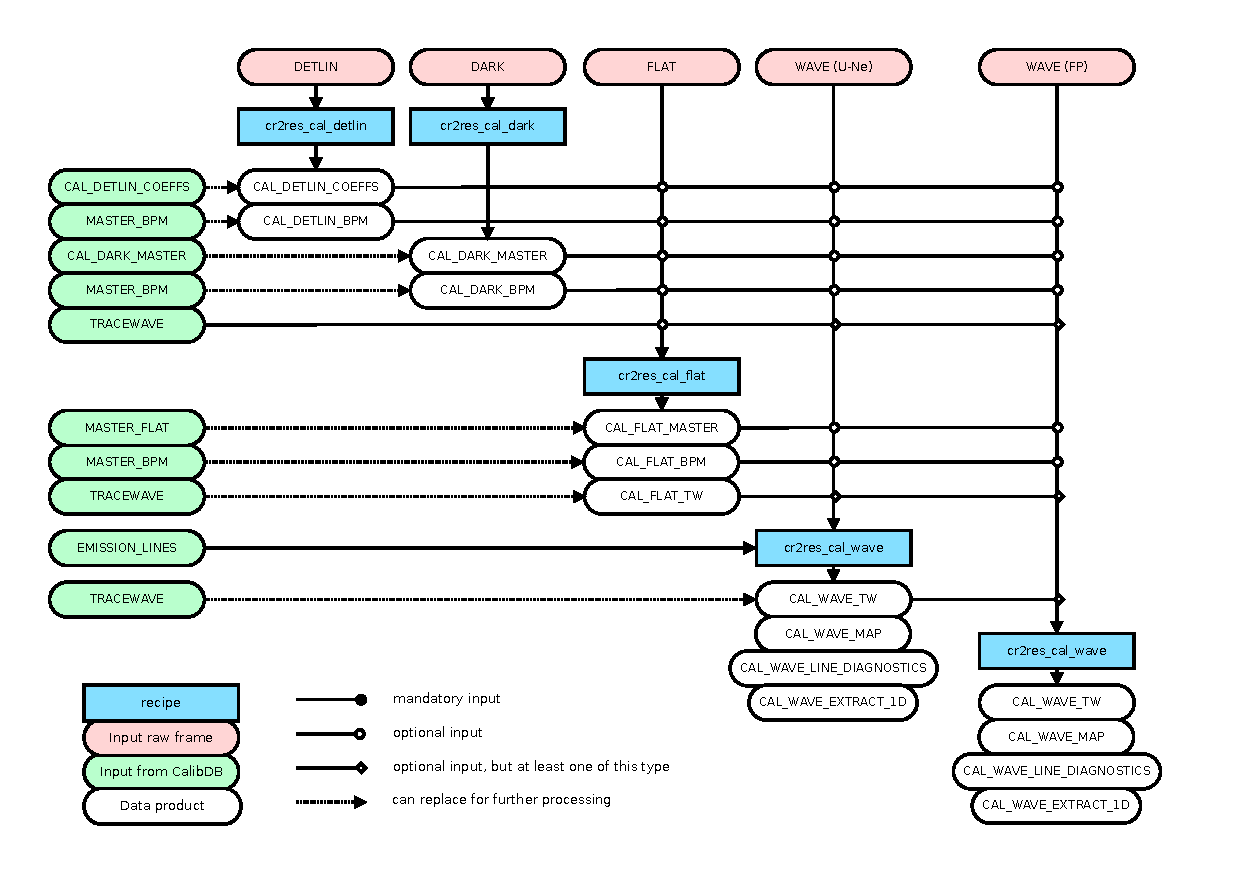
\includegraphics[width=0.99\linewidth]{calib_simple.pdf}
    \end{center}
    \caption{
        \label{fig:calibflow_simple}
        Flow diagram for calibration reduction with the \textit{calibration
        recipes}, assuming a populated CalibDB exists. Arrows and lines indicate
        the inputs to the recipes (blue), in the form of raw data (red), master
        calibrations from the CalibDB (green), or intermediate products from
        previous steps (white). Dash-dotted lines indicate when a CalibDB or
        intermediate product can be chosen for later steps further to the right.
        All line connections are optional (open symbols), but generally
        recommended being present. Also note that open diamonds mark TW inputs,
        of which at least one needs to be present.
    }
\end{figure}

Fig.~\ref{fig:calibflow_simple} shows how calibrations can be reduced in a way
that matches how the online (quick-look) reductions are run at the telescope.
For each type of calibration data there is a single recipe that processes them.
Apart from the raw frames, the necessary inputs can either come from the CalibDB
or from a previous step.


If a TW is provided to \texttt{cr2res\_cal\_flat}, it will use the information
therein; otherwise it performs the tracing of the spectral orders to find their
location. However, the slit tilt cannot be determined from flat-field frames
which means that the extraction of the blaze function will be done assuming a
vertical slit, yielding sub-optimal results in the bands Y-K. Therefore
providing a TW is recommended in these bands, either the one from the CalibDB,
or one made via \texttt{cr2res\_util\_trace} and
\texttt{cr2res\_util\_slit\_curv}.

Daily calibrations are taken with metrology turned on, and both the static
calibrations and the CalibDB at the telescope are derived from data with
metrology. This means that this way of reducing calibrations, relying on the
pre-existing TW for order locations and slit-tilt, is not expected to have
negative impact on the quality of data products, as long as the night-time
observations were also taken \emph{with} metrology.

Example SOFs and commands can be found in Ch.~\ref{sec:simcalexpl}.

\subsubsection{The step-by-step way}
\label{sec:stepcalib}

\begin{figure}[!tb]
    \begin{center}
        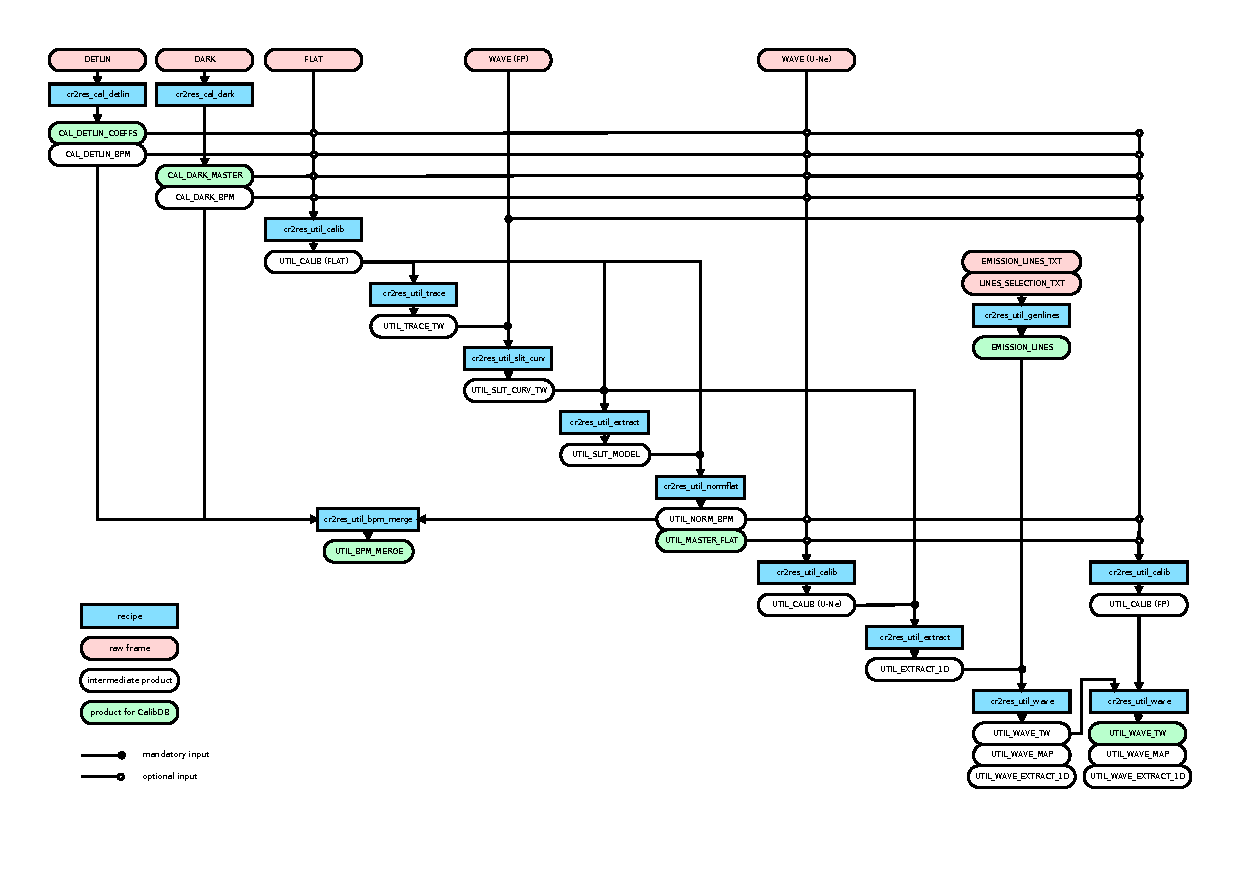
\includegraphics[width=0.99\linewidth]{calib_detailed.pdf}
    \end{center}
    \caption{
        \label{fig:calibflow_detailed}
        Flow diagram for calibration reduction with the \textit{utility
            recipes}, without relying on static calibrations. In other
            words, this is how the products for the CalibDB (green) can be made
            from scratch. Steps are numbered, but execution order can be changed
            whenever data flow allows. For notes on individual steps see main
            text.}
\end{figure}

Fig.~\ref{fig:calibflow_detailed} shows the calibration data flow step-by-step,
using the \emph{util} recipes that each only perform a single task. In addition,
no pre-existing calibrations are used, and it is in fact the way the
set of static calibrations is assembled in the first place.

A concrete example, using the same numbering of steps, is shown in
Ch.~\ref{sec:calibscratch}. Some aspects are worth pointing out first:

\begin{enumerate}
    \item \texttt{cr2res\_cal\_dark} combines the input DARK frames into a
    master dark for each setting and combination of DIT and NDIT. Hot and dead
    pixels get saved as BPM.
    \item \texttt{cr2res\_util\_calib} combines (\verb!--collapse=MEAN!)
    the raw FLAT frames and applies the	master dark and BPM.
    \item \texttt{cr2res\_util\_trace} finds continuous regions on the detectors
    that have signal, and fits them with polynomials for the orders' mid-lines
    and edges. These polynomials we call a \emph{trace} and each order can have
    more than one trace, e.g. marking different heights along the slit.
    \item \texttt{cr2res\_util\_slit\_curv} uses the TraceWave-table (TW) from
    the previous step to measure the lines in an FPET frame to determine
    how the slit tilt changes within each detector-order. The result is stored
    in an updated TW.
    \item \texttt{cr2res\_util\_extract} can now use this TW to extract the
    calibrated flat-field frame from step 2. This gives us the blaze
    spectrum (1D) and a 2D model of the frame.
    \item This model contains all non-local features, meaning that
    \texttt{cr2res\_util\_normflat} can calculate the \emph{normalized
    flat-field} through dividing the model by the original frame. Outliers in
    sensitivity get flagged as a BPM again.
    \item Next we use \texttt{cr2res\_util\_calib} once more, this time to merge the UNE frames and apply the calibrations from previous steps.
    \item Now \texttt{cr2res\_util\_extract} can collapse the result from the last step into 1D spectra.
    \item \texttt{cr2res\_util\_genlines} creates the catalog files for each
    setting, based on the base catalog and selection files that flag wavelength
    regions as usable for the setting at hand.
    \item[11.] \texttt{cr2res\_util\_wave} uses the spectra and catalog from the
    last two steps to derive a wavelength solution, i.e.~a polynomial
    that translates pixel-coordinates into wavelength (nm). Available methods
    include cross-correlation and line-fitting. This step can be repeated, for
    example to step-wise increase the polynomial degree.
    \item[13-15.] Analogous to steps 7-11 but for an FPET frame this time. The
    Etalon method of \texttt{cr2res\_util\_wave} will use the zero-point from
    the incoming TW and refine the higher degrees of the solution.
\end{enumerate}
